
\hspace{4mm}
Dans ce chapitre, nous commençons par une présentation de l'entreprise d'accueil "Mocalo". par la suite nous décrivons la problématique puis nous introduisons le cahier des charges de projet. Enfin, nous détaillons notre plan de travail.

\section{ Présentation de l’entreprise }

\hspace{4mm} MOCALO SERVICES est une société créée le 03 Octobre 2019, suite à un constat d’un fort besoin de conseils pour les entreprises de différents domaines. Elle est spécialisée dans le secteur d'activité de conseil en systèmes et logiciels informatiques.
\begin{figure}[h]
    \centering
    
\includegraphics[scale=0.2]{figures/aniskab.jpg}
    \caption{Logo Mocalo}
    \label{fig:logo_mocalo}
\end{figure}
\subsection{ 	Les rapports sociaux : }

\begin{itemize}
    \item	\textbf{Entre ouvriers :} Dans l’ensemble, les rapports sont amicaux et très entretenus. On avait l’habitude de venir 10 à 15 minutes avant l’heure de travail le matin pour avoir l’occasion de boire un café et discuter ensemble. 
\newpage    \item \textbf{Entre chefs et ouvriers :} Le schéma de base où le chef donne les ordres et l’ouvrier les exécute est rarement respecté dans l’entreprise. En effet, les ouvriers maitrisent leurs métiers et remplissent leurs fonctions avec les outils qu’ils ont et les chefs supervisent toutes les opérations et les valident.
\end{itemize}
\subsection{	Organigramme de l’entreprise  :}
\hspace{4mm}L’organigramme de la figure \ref{fig:bureau} montre une représentation schématique des liens hiérarchiques de l'organisme d'accueil. Il sert à donner une vue d’ensemble de la répartition des postes et fonctions au sein de l'entreprise. 
\begin{figure}[h]
		\centering
		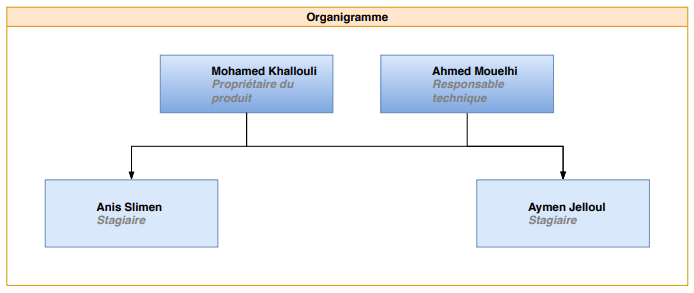
\includegraphics[scale=0.7]{figures/a10.png}
		\caption{Organigramme de l'entreprise}
		\label{fig:bureau}
\end{figure}

 \section{	Présentation du projet  }
 \subsection{	Problématique}
\hspace{4mm} Une des tendances les plus en vue et qui concerne tous les secteurs de développement informatique, est la numérisation. Depuis l’apparition de l’informatique et son introduction dans le monde économique, les entreprises et les entités publiques aspirent à optimiser et à rendre fiable la gestion de leurs structures internes.
\par A l’instar de toute entreprise, une SSII veut améliorer ses procédures de gestion des projets, pour disposer d’une vision globale des différents projets et de leurs états d’avancement.
\par Le succès d’un projet se mesure à la satisfaction du client et à la qualité du résultat, c’est-à-dire à la conformité du produit à ce qui est attendu et à sa livraison dans le respect du délai imparti et du budget alloué.
\par Au cours d’un projet, on est susceptible de confronter plusieurs risques à savoir:
\begin{itemize}
    \item Le risque de dépassement du budget.
    \item Le risque de dépassement des délais.
    \item Le risque d’abandon du projet.
\end{itemize}
\par Sans oublier le risque majeur qui peut toucher la gestion d'un projet et qui est l'absence ou la mauvaise communication entre les différents intervenants. 

\par ainsi pour dépasser tous les risques précédemment cités nous avons proposé une solution informatique à la fois simple, pratique et robuste.


\subsection{	Objectifs}
  \hspace{4mm}  Dans le cadre de mon projet de fin d’études en Génie logiciel, à l’Institut Supérieur des Sciences Appliquées et de Technologie de Sousse, je suis chargé de développer une application qui va servir de menu permettant d’effectuer des tâches spécifiques selon le profil de l’utilisateur.  
\par Chaque tâche devra répondre aux besoins de l’organisme comme par exemple établir un suivi de projet afin d’avoir une vision globale de l’avancement du projet. Il est aussi recommandé de mettre en place des recherches simples et multicritères pour effectuer des opérations d’ajout, de suppression et de modification sur les informations présentes dans la base de données définie préalablement.
\section{	Étude de l'existant}
\hspace{4mm} Nous ne saurions commencer ce travail et élaborer la solution proposée sans avoir une idée claire et précise sur l’existant. La première tâche dans notre projet était la recherche de ce qui est existant sur le marché numérique. Dans ce qui suit nous présentons quelques exemples d’applications ayant plus ou moins des fonctionnalités similaires à celles de notre projet dans le but de dégager leurs limites, ce qui va nous permettre de mettre en relief notre valeur ajoutée par rapport à ce qui existe déjà.

\begin{figure}[h]
		\centering
		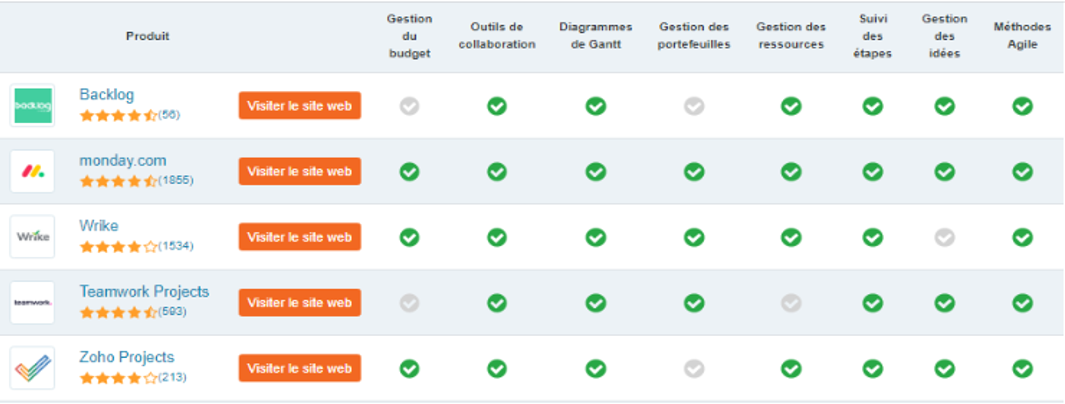
\includegraphics[scale=0.45]{figures/333ANIS3.png}
		\caption{Etude de l’existant}
		\label{fig:etudex}
\end{figure}\par Avant d’entamer une étude détaillée du projet, il nous a fallu réaliser une étude de l’existant sur le marché numérique ce qui nous a montré des insuffisances et plusieurs problèmes qui couvrent plusieurs préoccupations :
\begin{itemize}
    \item préoccupation en termes de rapidité : Comment accélérer le processus de travail au sein d’une entreprise de façon à gagner le maximum de temps ?
    \item préoccupation en termes d’accessibilité : Comment fournir aux utilisateurs un portail numérique simple et facile à exploiter ?
    \item Préoccupation en termes d’efficacité : Comment garantir une solution qui satisfait les besoins de l’utilisateur ?
\end{itemize}
\section{Solution proposée}

\hspace{4mm}    Notre solution consiste à développer une plateforme web de gestion de projets. Cette plateforme permet, d’une manière centralisée, d’aider les sociétés de services à la gestion des tâches, notamment au suivi de projets, du temps et de la collaboration en équipes. 

\section{	Chronologie}
\hspace{4mm}La planification est parmi les phases d'avant-projet. Elle consiste non seulement à délimiter le périmètre temporel du projet, mais aussi à prévoir le déroulement des activités tout au long de la période allouée au stage. La figure suivante détaille la planification temporelle du projet :
% \begin{center}
% \begin{tabular}{|c|l|l|l|l|l|l|l|l|l|l|}
% \hline 
% Produit & Gestion  & Outils de  & Diagramme  & Gestion des  & Gestion des  & suivi des  & Gestion  & Méthodes \\&de budget&collaboration&de Gantt&portfeuilles&ressources&étapes&des idées&Agile
% \\\hline 
%     Backlog &%
\includegraphics{figures/aniska.png}
% & & & & & & &\\\hline 
%     monday.com & & & & & & & & \\\hline
%     Wrike & & & & & & & & \\\hline 
%     Teamwork Projects & & & & & & & & \\\hline 
    
% \end{tabular}
% \captionof{table}{Description du processus de l’authentification}
% \label{desc_auth}
% \end{center}

\begin{figure}[h]
		\centering
		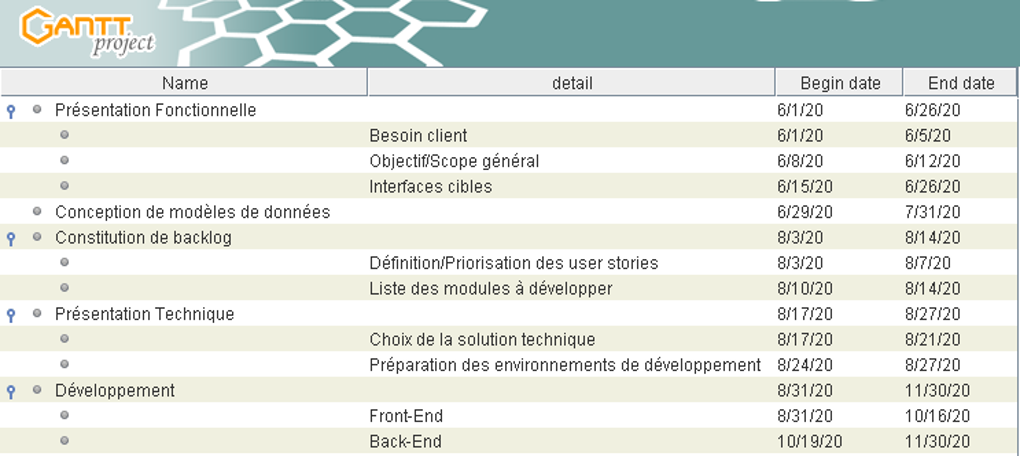
\includegraphics[scale=0.9]{figures/anis3.png}
		\caption{Diagramme de GANTT}
		\label{fig:gantt}
\end{figure}
\section{	Processus de développement}
\hspace{4mm}Agile est un ensemble de méthodes et de processus, orienté collaboratif, transversalité et autonomie ; dont les grands principes sont notamment exposés dans le manifeste Agile.
\par Parmi les méthodologies agiles les plus utilisées est Scrum que nous avons choisie d'utiliser pour notre projet. 
\par La méthodologie scrum, offre plusieurs avantages : Elle assure la livraison de l’application dans les bons délais, tout en fournissant un produit qui respecte les attentes du client. Cela, nous permet d’obtenir une application plus flexible qui s’adapte plus facilement aux nouveaux changements.\newpage



\section*{Conclusion}
\hspace{4mm} Ce chapitre est considéré comme la partie introductive de notre projet, dont laquelle nous avons dégagé la problèmatique , ensuite nous avons récapitulé une idée générale sur les différentes applications existantes ayant plus ou moins des fonctionnalités similaires à celles de notre projet et enfin nous avons présenté notre solution. Le chapitre suivant présentera la spécification des besoins afin d'atteindre les objectifs fixés pour notre projet.

	

